%
% Main document
% ===========================================================================
% This is part of the document "Project documentation template".
% Authors: brd3, kaa1
%
%---------------------------------------------------------------------------
\documentclass[
    a4paper,                    % paper format
    10pt,                           % fontsize
    %twoside,                    % double-sided
    openright,              % begin new chapter on right side
    notitlepage,            % use no standard title page
    parskip=half,           % set paragraph skip to half of a line
]{scrreprt}                 % KOMA-script report
%---------------------------------------------------------------------------
\raggedbottom{}
%\KOMAoptions{cleardoublepage=plain}         % Add header and footer on blank pages


% Load Standard Packages:
%---------------------------------------------------------------------------
\usepackage[standard-baselineskips]{cmbright}

\usepackage[ngerman]{babel}                                             % german hyphenation
\usepackage[utf8]{inputenc}                                             % UTF-8 input encoding
\usepackage[T1]{fontenc}                                                % hyphenation of words with ä,ö and ü
\usepackage{textcomp}                                                   % additional symbols
\usepackage{ae}                                                         % better resolution of Type1-Fonts 
\usepackage{fancyhdr}                                                   % simple manipulation of header and footer 
\usepackage{etoolbox}                                                   % color manipulation of header and footer
\usepackage{graphicx}                                                   % integration of images
\usepackage{float}                                                      % floating objects
\usepackage{caption}                                                    % for captions of figures and tables
\usepackage{booktabs}                                                   % package for nicer tables
\usepackage{tocvsec2}                                                   % provides means of controlling the sectional numbering
\usepackage[square,sort,comma,numbers]{natbib}                          % provides various citation styles
\usepackage{wrapfig}                                                    % provides floating of text around images
%---------------------------------------------------------------------------

% Load Math Packages
%---------------------------------------------------------------------------
\usepackage{amsmath}                                                    % various features to facilitate writing math formulas
\usepackage{amsthm}                                                     % enhanced version of latex's newtheorem
\usepackage{amsfonts}                                                   % set of miscellaneous TeX fonts that augment the standard CM
\usepackage{amssymb}                                                    % mathematical special characters
\usepackage{exscale}                                                    % mathematical size corresponds to textsize
%---------------------------------------------------------------------------

% Package to facilitate placement of boxes at absolute positions
%---------------------------------------------------------------------------
\usepackage[absolute]{textpos}
\setlength{\TPHorizModule}{1mm}
\setlength{\TPVertModule}{1mm}
%---------------------------------------------------------------------------                    
            
% Definition of Colors
%---------------------------------------------------------------------------
\RequirePackage{color}                          % Color (not xcolor!)
\definecolor{linkblue}{rgb}{0,0,0.8}            % Standard
\definecolor{darkblue}{rgb}{0,0.08,0.45}        % Dark blue
\definecolor{bfhgrey}{rgb}{0.41,0.49,0.57}      % BFH grey
%\definecolor{linkcolor}{rgb}{0,0,0.8}              % Blue for the web- and cd-version!
\definecolor{linkcolor}{rgb}{0,0,0}                 % Black for the print-version!
%---------------------------------------------------------------------------

% Hyperref Package (Create links in a pdf)
%---------------------------------------------------------------------------
\usepackage[
    pdftex,ngerman,bookmarks,plainpages=false,pdfpagelabels,
    backref = {false},                                      % No index backreference
    colorlinks = {true},                  % Color links in a PDF
    hypertexnames = {true},               % no failures "same page(i)"
    bookmarksopen = {true},               % opens the bar on the left side
    bookmarksopenlevel = {0},             % depth of opened bookmarks
    pdftitle = {Template für Bachelor Thesis},      % PDF-property
    pdfauthor = {brd3},                           % PDF-property
    pdfsubject = {LaTeX Template},        % PDF-property
    linkcolor = {linkcolor},              % Color of Links
    citecolor = {linkcolor},              % Color of Cite-Links
    urlcolor = {linkcolor},               % Color of URLs
]{hyperref}
%---------------------------------------------------------------------------
% Set up page dimension
%---------------------------------------------------------------------------
\usepackage{geometry}
\geometry{a4paper,
    left=28mm,
    right=15mm,
    top=30mm,
    headheight=20mm,
    headsep=10mm,
    textheight=242mm,
    footskip=15mm
}
%---------------------------------------------------------------------------

% Makeindex Package
%---------------------------------------------------------------------------
\usepackage{makeidx}                                % To produce index
\makeindex                                      % Index-Initialisation
%---------------------------------------------------------------------------

% Glossary Package
%---------------------------------------------------------------------------
% the glossaries package uses makeindex
% if you use TeXnicCenter do the following steps:
%  - Goto "Ausgabeprofile definieren" (ctrl + F7)
%  - Select the profile "LaTeX => PDF"
%  - Add in register "Nachbearbeitung" a new "Postprozessoren" point named Glossar
%  - Select makeindex.exe in the field "Anwendung" ( ..\MiKTeX x.x\miktex\bin\makeindex.exe )
%  - Add this [ -s "%tm.ist" -t "%tm.glg" -o "%tm.gls" "%tm.glo" ] in the field "Argumente"
%
% for futher informations go to http://ewus.de/tipp-1029.html
%---------------------------------------------------------------------------
\usepackage[nonumberlist]{glossaries}
%\usepackage[xindy,nonumberlist]{glossaries}

% das zügs do unde dra find i eigendli unnötig, wenn mir so afön fülle mir sitewiss mit "`unüebliche"' begriffe! :(
\newglossaryentry{UML}{name={Wissensmodellierung},description={...}}
\newglossaryentry{Relationale Datenbank}{name={Beschreibungslogik },description={Reasoner ...}}
\newglossaryentry{Relationale Datenspeicherung}{name={Beschreibungslogik },description={Reasoner ...}}
\newglossaryentry{Semantische Datenbank}{name={Beschreibungslogik },description={Reasoner ...}}
\newglossaryentry{Expertensystem}{name={Beschreibungslogik },description={Reasoner ...}}
\newglossaryentry{Ontologie}{name={Ontologie},description={...}}
\newglossaryentry{Domäne}{name={Beschreibungslogik },description={Reasoner ...}}
\newglossaryentry{Wissensdomäne}{name={Beschreibungslogik },description={Reasoner ...}}
\newglossaryentry{Problemdomäne}{name={Beschreibungslogik },description={Reasoner ...}}
\newglossaryentry{Reasoner}{name={Beschreibungslogik },description={Reasoner ...}}
\newglossaryentry{Inferenzmaschine}{name={Beschreibungslogik },description={Reasoner ...}}
\newglossaryentry{Tutorial}{name={Beschreibungslogik },description={Reasoner ...}}
\newglossaryentry{RDF/XML}{name={Resolution},description={...}}
\newglossaryentry{OWL/XML}{name={Parser },description={...}}

\newglossaryentry{Semantik}{name={Inferenz},description={...}}
\newglossaryentry{Knowledge-Engineering}{name={Wissensmodellierung},description={...}}
\newglossaryentry{Knowledge-Engineer}{name={Wissensingeneur},description={Analytiker, Informationsmanager mit entsprechender Methodik und entsprechenden Werkzeugen}}
\newglossaryentry{HERMES}{name={Resolution},description={...}}
\newglossaryentry{Scrum}{name={Inferenz},description={...}}
\newglossaryentry{RDF}{name={Resolution},description={...}}
\newglossaryentry{OWL}{name={Inferenz},description={...}}
\newglossaryentry{Ontologie-Sprache}{name={Inferenz},description={...}}
\newglossaryentry{SWRL}{name={Inferenz},description={...}}
\newglossaryentry{SPARQL}{name={Inferenz},description={...}}
\newglossaryentry{W3C}{name={Inferenz},description={...}}
\newglossaryentry{Apache Stanbol}{name={Inferenz},description={...}}
\newglossaryentry{Stanford Protégé}{name={Inferenz},description={...}}
\newglossaryentry{Clark & Parsia Stardog}{name={Inferenz},description={...}}
\newglossaryentry{XML}{name={Inferenz},description={...}}
\newglossaryentry{Graphdatenbank}{name={Beschreibungslogik },description={Reasoner ...}}
\newglossaryentry{yWorks yEd}{name={Beschreibungslogik },description={Reasoner ...}}
\newglossaryentry{Unifikation}{name={Beschreibungslogik },description={Reasoner ...}}
\newglossaryentry{Semantisches Netz}{name={Parser },description={...}}
\newglossaryentry{NP-vollständig}{name={Parser },description={...}}
\newglossaryentry{URL}{name={Parser },description={...}}
\newglossaryentry{Turtle}{name={Parser },description={...}}
\newglossaryentry{FACT++}{name={Parser },description={...}}
\newglossaryentry{Pellet}{name={Beschreibungslogik },description={Reasoner ...}}
\newglossaryentry{SNARL}{name={Beschreibungslogik },description={Reasoner ...}}
%bis 6.2.1 ok
\newglossaryentry{Resolution}{name={Resolution},description={...}}
\newglossaryentry{Inferenz}{name={Inferenz},description={...}}

\newglossaryentry{Wissensakquise}{name={Wissensakquise},description={Sammeln/ erfassen, aufarbeiten/strukturieren von Wissen}}
\newglossaryentry{Parser}{name={Parser },description={...}}

\newglossaryentry{Beschreibungslogik}{name={Beschreibungslogik },description={Reasoner ...}}
\newglossaryentry{Frame}{name={Parser },description={...}}
\newglossaryentry{Wissensnetzte }{name={Parser },description={...}}

\newglossaryentry{Konzepte}{name={Parser },description={...}}
\newglossaryentry{Axiome}{name={Parser },description={...}}
\newglossaryentry{Prinzipien}{name={Parser },description={...}}
\newglossaryentry{Wissensmodellierung}{name={Beschreibungslogik },description={Reasoner ...}}

\newglossaryentry{Semantisches Web}{name={Beschreibungslogik },description={Reasoner ...}}
\newglossaryentry{Semantik}{name={Beschreibungslogik },description={Reasoner ...}}
\newglossaryentry{Formale Sprache}{name={Beschreibungslogik },description={Reasoner ...}}
\newglossaryentry{Künstliche Intelligenz}{name={Beschreibungslogik },description={Reasoner ...}}
\newglossaryentry{Aussagenlogik}{name={Beschreibungslogik },description={Reasoner ...}}
\newglossaryentry{Prädikatenlogik}{name={Beschreibungslogik },description={Reasoner ...}}

\newglossaryentry{Hierarchische Datenbank}{name={Beschreibungslogik },description={Reasoner ...}}
%\newglossaryentry{Graph}{name={Beschreibungslogik },description={Reasoner ...}}
%\newglossaryentry{Zyklenfreie Nachbarschaft}{name={Beschreibungslogik },description={Reasoner ...}}
%\newglossaryentry{Entität}{name={Beschreibungslogik },description={Reasoner ...}}
%\newglossaryentry{Knoten}{name={Beschreibungslogik },description={Reasoner ...}}
%\newglossaryentry{Kanten}{name={Beschreibungslogik },description={Reasoner ...}}
\newglossaryentry{Existenzaussage}{name={Beschreibungslogik },description={Reasoner ...}}
\newglossaryentry{Ontologiesprache}{name={Beschreibungslogik },description={Reasoner ...}}

\newglossaryentry{Modus Ponens}{name={Beschreibungslogik },description={Reasoner ...}}
\newglossaryentry{Theorem}{name={Beschreibungslogik },description={Reasoner ...}}

\newglossaryentry{Tableau-Kalkül}{name={Beschreibungslogik },description={Reasoner ...}}
\newglossaryentry{Prämisse}{name={Beschreibungslogik },description={Reasoner ...}}
\newglossaryentry{Konklusion}{name={Beschreibungslogik },description={Reasoner ...}}
\newglossaryentry{Literal}{name={Beschreibungslogik },description={Reasoner ...}}
\newglossaryentry{xxx}{name={Beschreibungslogik },description={Reasoner ...}}


\makeglossaries{}
%---------------------------------------------------------------------------

% Intro:
%---------------------------------------------------------------------------
%\begin{document}                                % Start Document
\settocdepth{section}                                                       % Set depth of toc
\pagenumbering{roman}                                                       
%---------------------------------------------------------------------------

\providecommand{\titel}{Titel des Berichts}		%  Hier den Titel des Berichts/Thesis eingeben                  % Titel der Arbeit aus Datei titel.tex lesen
\providecommand{\versionnumber}{0.1}			%  Hier die aktuelle Versionsnummer eingeben
\providecommand{\versiondate}{08.06.2014}		%  Hier das Datum der aktuellen Version eingeben
                % Versionsnummer und -datum aus Datei version.tex lesen

% Set up header and footer
%---------------------------------------------------------------------------
\makeatletter
\patchcmd{\fancyhead}{\rlap}{\color{bfhgrey}\rlap}{}{}     % new color of header
\patchcmd{\fancyfoot}{\rlap}{\color{bfhgrey}\rlap}{}{}     % new color of footer
\makeatother

\fancyhf{}                                                                      % clean all fields
\fancypagestyle{plain}{% new definition of plain style 
    \fancyfoot[OR,EL]{\footnotesize \thepage}   % footer right part --> page number
    \fancyfoot[OL,ER]{\footnotesize \titel, Version \versionnumber, \versiondate}   % footer even page left part 
}

\renewcommand{\chaptermark}[1]{\markboth{\thechapter.  #1}{}}
\renewcommand{\headrulewidth}{0pt}              % no header stripline
\renewcommand{\footrulewidth}{0pt}              % no bottom stripline

\pagestyle{plain}
%---------------------------------------------------------------------------

\begin{document}

% Title Page and Abstract
%---------------------------------------------------------------------------
%%
% Project documentation template
% ===========================================================================
% This is part of the document "Project documentation template".
% Authors: brd3, kaa1
%

\begin{titlepage}


% BFH-Logo absolute placed at (28,12) on A4 
% Actually not a realy satisfactory solution but working.
%---------------------------------------------------------------------------
\setlength{\unitlength}{1mm}
\begin{textblock}{20}[0,0](28,12)
	
\includegraphics[scale=1.0]{bilder/BFH_Logo_B.png}
\end{textblock}
\color{black}

% Institution / Titel / Untertitel / Autoren / Experten:
%---------------------------------------------------------------------------
\begin{flushleft}

\vspace*{21mm}

\fontsize{26pt}{40pt}\selectfont 
\titel 				\\							% Titel aus der Datei vorspann/titel.tex lesen
\vspace{2mm}

\fontsize{16pt}{24pt}\selectfont\vspace{0.3em}
Hier steht ein Untertitel 			\\							% Untertitel eingeben
\vspace{5mm}

\fontsize{10pt}{12pt}\selectfont
\textbf{Art der Arbeit (Semesterarbeit / Bachelorthesis / etc.)} \\									% eingeben
\vspace{7mm}

% Abstract (eingeben):
%---------------------------------------------------------------------------
\begin{textblock}{150}(28,100)
\fontsize{10pt}{12pt}\selectfont
[Kurztext (Abstract) einf�gen, falls gew�nscht] \\ 
Dieses Dokument dient als Vorlage f�r die Erstellung von Berichten nach den Richtlinien der BFH. Die Vorlage ist in \LaTeX{} erstellt und unterst�tzt das automatische Erstellen von diversen Verzeichnissen, Literaturangaben, Indexierung und Glossaren. Dieser kleine Text ist eine Zusammenfassung �ber das vorliegenden Dokument mit einer L�nge von 4 bis max. 8 Zeilen. \\
Das Titelbild kann in den Zeilen 157/158 der Datei template.tex ein- oder ausgeschaltet werden.
\end{textblock}

\begin{textblock}{150}(28,225)
\fontsize{10pt}{17pt}\selectfont
\begin{tabbing}
xxxxxxxxxxxxxxx\=xxxxxxxxxxxxxxxxxxxxxxxxxxxxxxxxxxxxxxxxxxxxxxx \kill
Studiengang:	\> [z.B. Elektro- und Kommunikationstechnik]	\\			% Namen eingeben
Autoren:		\> [Test Peter, M�ster R�s�]		\\					% Namen eingeben
Betreuer:	\> [Dr.~Xxxx Xxxx, Dr.~Yyyy Yyyy]		\\					% Namen eingeben
Auftraggeber:	\> [Wwwww AG]						\\					% Namen eingeben
Experten:		\> [Dr.~Zzzz Zzzz]				\\					% Namen eingeben
Datum:			\> \versiondate					\\		% aus Datei vorspann/version.tex lesen
\end{tabbing}

\end{textblock}
\end{flushleft}

\begin{textblock}{150}(28,280)
\noindent 
\color{bfhgrey}\fontsize{9pt}{10pt}\selectfont
Berner Fachhochschule | Haute �cole sp�cialis�e bernoise | Bern University of Applied Sciences
\color{black}\selectfont
\end{textblock}


\end{titlepage}

%
% ===========================================================================
% EOF
%
        % activate for Titelseite ohne Bild
%
% Project documentation template
% ===========================================================================
% This is part of the document "Project documentation template".
% Authors: brd3, kaa1
%

\begin{titlepage}


% BFH-Logo absolute placed at (28,12) on A4 and picture (16:9 or 15cm x 8.5cm)
% Actually not a realy satisfactory solution but working.
%---------------------------------------------------------------------------
\setlength{\unitlength}{1mm}
\begin{textblock}{20}[0,0](28,12)
    
\includegraphics[scale=1.0]{bilder/BFH_Logo_B.png}
\end{textblock}

\begin{textblock}{154}(28,48)
    \begin{picture}(150,2)
        \put(0,0){\color{bfhgrey}\rule{150mm}{2mm}}
    \end{picture}
\end{textblock}

\begin{textblock}{154}[0,-0.2](28,42)
    \centering
    
\includegraphics[scale=0.7]{bilder/owl.png}   % Titelbild definieren
\end{textblock}

\begin{textblock}{154} (28,135)
    \begin{picture}(150,2)
        \put(0,0){\color{bfhgrey}\rule{150mm}{2mm}}
    \end{picture}
\end{textblock}
\color{black}

% Institution / Titel / Untertitel / Autoren / Experten:
%---------------------------------------------------------------------------
\begin{flushleft}

\vspace*{120mm}

\fontsize{26pt}{28pt}\selectfont
\titel% Titel aus der Datei vorspann/titel.tex lesen
\vspace{3mm}



\fontsize{10pt}{12pt}\selectfont
\textbf{Aufbau von Wissensdomänen anhand einer semantischen Datenbank} \\                                 % eingeben
\vspace{3mm}

\begin{textblock}{150} (28,215)
\fontsize{10pt}{17pt}\selectfont
\begin{tabbing}
xxxxxxxxxxxxxxx\=xxxxxxxxxxxxxxxxxxxxxxxxxxxxxxxxxxxxxxxxxxxxxxx \kill
Autoren:        \> Sven Osterwalder, Mira Günzburger     \\                  % Namen eingeben
Datum:          \> \versiondate\\      % aus Datei vorspann/version.tex lesen
\end{tabbing}

\end{textblock}
\end{flushleft}

\begin{textblock}{150} (28,280)
\noindent 
\color{bfhgrey}\fontsize{9pt}{10pt}\selectfont
Berner Fachhochschule | Haute école spécialisée bernoise | Bern University of Applied Sciences
\color{black}\selectfont
\end{textblock}


\end{titlepage}

%
% ===========================================================================
% EOF
%
          % activate for Titelseite mit Bild
% Versionenkontrolle :
% -----------------------------------------------

\begin{textblock}{180} (15,150)
\color{black}
\begin{huge}
Versionen
\end{huge}
\vspace{10mm}

\fontsize{10pt}{18pt}\selectfont
\begin{tabbing}
xxxxxxxxxxx\=xxxxxxxxxxxxxxx\=xxxxxxxxxxxxxx\=xxxxxxxxxxxxxxxxxxxxxxxxxxxxxxxxxxxxxxxxxxxxxxx \kill
Version	\> Datum	\> Status		\> Bemerkungen		\\
0.1	\> 08.06.2014	\> Entwurf		\> Anforderungsdokument erstellen	\\	
0.2	\> 08.08.2014	\> Entwurf		\> Korrekturen und Ergänzungen	\\	
0.3	\> 19.09.2014	\> Entwurf		\> Anpassungen an die Aufgabenstellung	\\ 
%0.3	\> 02.09.2013	\> Entwurf		\> Donec eget aliquam urna. Lorem ipsum dolor sit amet	\\ 
%1.0	\> 12.09.2013	\> Definitiv	\> Lorem ipsum dolor sit ametPhasellus scelerisque, leo sed iaculis ornare 	\\ 
%1.1	\> 04.11.2013	\> Korrektur	\> Layout angepasst	\\
\end{tabbing}

\end{textblock}

%\cleardoubleemptypage{}
\setcounter{page}{1}
\cleardoublepage{}
\phantomsection{}
\addcontentsline{toc}{chapter}{Management Summary}
\chapter*{Management Summary}
\label{chap:management_summary}

\cleardoubleemptypage
%---------------------------------------------------------------------------

% Table of contents
%---------------------------------------------------------------------------
\tableofcontents
%\cleardoubleemptypage
%\cleardoublepage
%---------------------------------------------------------------------------

% Main part:
%---------------------------------------------------------------------------
\pagenumbering{arabic}
\chapter{Einleitung}
\label{chap:einleitung}

%CHeckliste fausibibel
%Ausgangslage, Problemstellung
%• Auftrag oder Aufgabenstellung
%• Resultat der Arbeit
%• Methodik (Herkunft der Daten, Vorgehen, Systemund
%Gültigkeitsgrenzen)
%• Folgerungen, offene Fragen

Der klassische Ansatz der Wissensabbildung, zum Beispiel in Form von UML, welchem die relationale Datenspeicherung zugrunde liegt, wird in der heutigen Informatik weitläufig eingesetzt und ist de facto Standard. Häufig geschieht dies in enger Verbindung mit der objektorientierten Programmierung. Experten aus einer Fachrichtung sind fähig diese Daten zu interpretieren und daraus Schlüsse zu ziehen. Es ist aber nicht möglich automatisch Fragestellungen zu beantworten, welche über reine Relationsverknüpfungen hinausgehen. Mit dieser Technik sind Objekteigenschaften und -Verhalten also eher schwer abbildbar. Eine andere Art Wissen zu repräsentieren sind semantische Datenbanken. Diese ermöglichen das Abbilden des Objektverhaltens und können mithilfe von Schlussfolgerungen die Rolle des Experten einnehmen.

In dieser Bachelorthesis soll eine solche semantische Datenbank aufgebaut und angewendet werden.  Die Arbeit wurde in zwei Teilen umgesetzt: Einem  theoretischen und einem praktischen Teil. Der theoretische Teil zeigt in Form eines Tutorials auf, wie ein knowledge engineer bei der Wissensmodellierung vorgeht. Er nutzt dabei Ontologien als Basis, um eine semantische Datenbank aufzubauen. Im praktischen Teil soll eine solche Ontologie aufgebaut und per Benutzerschnittstelle zugänglich gemacht werden.

Die gesteckten Ziele konnten allesamt erreicht werden. Es ist den Autoren gelungen die Theorie der Wissensmodellierung übersichtlich in einem Dokument aufzubereiten und wiederzugeben. Speziell dabei ist, dass in diesem fachliche Grundlagen mit einem praktischen Beispiel verbunden werden. Zusätzlich konnten auch konkrete Tipps aus der eigenen Erfahrung eingeflochten werden. Dieses Dokument ist dem Abschlussdokument als Anhang beigefügt.

Im praktischen Teil der Arbeit wurde ein Expertensystem für Reisen aufgebaut: ``In der heutigen Zeit werden Ferien häufig per Internet gebucht. Was aber, wenn der Urlaub nicht einfach zwei Wochen an einem Ort stattfinden soll? Was, wenn der Kunde reisen möchte? Oder sonstige spezielle Wünsche hat? Für solche Anforderungen muss er auch heute noch in ein Reisebüro um sich beraten zu lassen.''\\
Bei der Automatisierung dieses Prozesses kommt die Ontologie ins Spiel, welche mithilfe von Eigenschaften, Kriterien und Regeln die Problemdomäne abbildet. Durch die Verwendung eines Reasoners können verschiedene Reisevorschläge gemacht werden.\\
Um eine sehr individuelle Reiseplanung zu erreichen, musste zuerst eine Ontologie in Form von Klassen, Individuen, Relationen und Eigenschaften erstellt werden. Ohne klaren Rahmen würde eine Ontologie zu komplex und zu gross. Daher bauten die Autoren die Ontologie anhand exemplarischer Tages und Wochenendausflügen in der Schweiz auf.\\
Als Ergebnis können die Autoren eine semantischen Datenbank präsentieren. Dabei wird die von ihnen gewählte Problemdomäne in einem klar gesteckten Rahmen abgedeckt und die Mächtigkeit der Wissensmodellierung veranschaulicht. Die Schnittstelle für Benutzer wurde in Form eines Assistenten umgesetzt, welcher den Benutzer durch die Möglichkeiten führt und ihn bei der Planung seiner Reise unterstützt. Damit konnten die Autoren verhindern, dass Benutzer gezwungen sind, Abfragen in einer komplexen Abfragesprache zu formulieren.

Die Wissensmodellierung auf Basis von Ontolgien ist auf ihre Weise eine mächtiges Werkzeug um Informationen mit Semantik zu versehen. Trotzdem hat diese Art der Modellierung gewisse Einschränkungen, welche von anderen auf Logik basierenden Sprachen, wie zum Beispiel Prolog, abgedeckt werden. Im Laufe der Arbeit erkannten die Autoren, dass es noch Bedarf an Weiterentwicklung im Bezug auf die angebotenen Werkzeuge gibt. So musste eine Kombination von zwei Werkzeugen verwendet werden um sämtliche Anforderungen umzusetzen.

% Hier beschreiben Sie kurz das Thema der Arbeit, den Kontext sowie in knappen Worten das Ergebnis. Dieser Abschnitt gleicht einem Management Summary. Ziel dieses Kapitels ist, dem Leser die Entscheidungsgrundlage zu liefern, ob er die Arbeit lesen soll oder nicht.

% Einträge im Verzeichnis erscheinen lassen ohne hier eine Referenz einzufügen
%\nocite{kopka:band1}

\chapter{Aufgabenstellung}
\label{chap:Aufgabenstellung}

% In diesem Kapitel wir die Aufgabenstellung beschrieben. Erwähnt werden soll die Ausgangslage (was hat es schon gegeben, was ist schon gemacht worden), auf der die Arbeit aufbaut. Im weiteren wird das Ziel beschrieben, welches erreicht werden soll. Daraus leitet sich das in dieser Arbeit gelöste Problem ab.

"`Ziel dieser Arbeit ist die Entwicklung und Anwendung eines Systems zur Speicherung in einer Semantischen Datenbank auf der Basis von Apache Stanbol. Dies schliesst die Erstellung einer Domänen-Ontologie mittels RDF/OWL ein und die Anwendung dieser Ontologie auf ein Anwendungsproblem, wie beispielsweise der Erlernung einer Programmiersprache ein. Exemplarisch soll aufgezeigt werden, wie dabei ein Knowledge Engineer vorgehen, um eine Problemdomäne systematisch zu modellieren und formalisieren. Besondere Bedeutung kommt dabei der Schnittstelle zwischen Mensch und System zu."'~\cite{Aufgabenstellung}


\chapter{Vorgehen}
\label{chap:vorgehen}

% Dieses Kapitel beschreibt das methodische Vorgehen, welches in der Arbeit angewendet wurde. Erwähnen Sie hier die verschiedenen Phasen der Arbeit und ihre Ergebnisse. Arbeiten mit hohem Softwareentwicklungs-Anteil lehnen sich am besten an eine etablierte Vorgehensweise an wie zum Beispiel Scrum, XP oder Agiler UP. Detailierte Projektpläne, Deliverables und anderes, falls vorhanden, gehören aber in den Anhang.

\section{Arbeitsorganisation}
\label{sec:vorgehen_orga}

Bei dieser Diplomarbeit steht, wie bereits erwähnt, der Prozess der Entstehung eines Expertensystems und der Analyse der dazugehörigen Grundlagen im Vordergrund. Der Anteil an Softwareentwicklung steht daher bewusst nicht im Fokus. Aus diesem Grund wurde keine der traditionellen Methoden der Projektorganisation gewählt.
Als Grundlage der Organisation dienten die im Voraus definierten Meilensteine. Zu jedem dieser Meilensteine wurde ein Endtermin sowie eine individuelle Liste von Tätigkeiten festgelegt. Anhand der Liste wurden die Arbeiten auf die zwei Autoren verteilt.

Der benötigte Zeitaufwand sowie die jeweiligen Arbeiten wurden in einem gemeinsamen Journal erfasst. Ein wichtiger Teil der Arbeit war ein Dokument, welches gewonnene Erkenntnisse festhält. In diesem wurden sämtliche Erfolge und Misserfolge beschrieben und analysiert. Dieses Dokument diente als Grundlage für das hier vorliegende Abschlussdokument.

\subsection{Regelmässige Treffen}
\label{sec:vorgehen_orga_treffen}
Zur Einhaltung der gesteckten Ziele und um ein Entwicklung in die falsche Richtung zu vermeiden, wurden regelmässige Treffen mit dem Betreuer der Arbeit abgehalten. Der Betreuer unterstützte die Autoren dabei mit Ideen. Die Treffen wurden im Minimum alle zwei Wochen abgehalten.

\section{Projektphasen}
\label{sec:projektphasen}

\subsection{Meilensteine}
\label{subsec:vorgehen_projektphasen_meilensteine}
Um bei der Arbeit ein möglichst strukturiertes Vorgehen einzuhalten, wurden folgende Projektphasen gewählt:
\begin{itemize}
    \item Projektstart
    \item Erarbeitung und Festhalten der Anforderungen
    \item Erarbeitung der formalen und technischen Grundlagen
    \item Modellierung der Ontologie
    \item Erstellung der Dokumentation zur Wissensmodellierung (Tutorial)
    \item Erstellung des Prototypen der Benutzerschnittstelle
    \item Erstellung der abschliessenden Dokumentation
\end{itemize}

Die erarbeiteten Grundlagen wurden in das Tutorial eingearbeitet und konnten direkt zur praktischen Umsetzung des Modells verwendet werden. Die aus der Modellierung gewonnen Erkenntnisse konnten wiederum direkt in das Dokument übernommen werden. Die verschiedenen Phasen liefen dabei parallel ab.

\subsection{Zeitplan}
\label{subsec:vorgehen_projektphasen_zeitplan}

\begin{figure}[H]
    \begin{ganttchart}[
        vgrid,
        x unit=0.7cm,
        bar/.append style={fill=bfhgrey!50},
    ]{1}{16}
        \gantttitle{2014}{14}
        \gantttitle{2015}{2} \\
        \gantttitlelist{1,...,16}{1} \\ % chktex 11
        \ganttbar{Projektstart}{1}{2} \\
        \ganttbar{Anforderungen}{1}{3} \\
        \ganttbar{Erarbeitung Grundlagen}{1}{10} \\
        \ganttbar{Tutorialdokument}{4}{5} \ganttbar{}{8}{14} \\
        \ganttbar{Modellierung Ontologie}{5}{8} \ganttbar{}{10}{14}\\
        \ganttbar{Umsetzung Prototyp}{9}{14} \\
        \ganttbar{Dokumentation}{1}{2} \gaanttbar{}{9}{16} \\
        \ganttbar{Präsentation/Verteidigung vorbereiten}{}{13}{16}

        % \ganttlink{elem1}{elem2}
        % \ganttlink{elem1}{elem2}
        % \ganttlink{elem2}{elem3}
        % \ganttlink{elem3}{elem4}
        % \ganttlink{elem4}{elem8}
    \end{ganttchart}
    \caption{Zeitplan; Der Titel stellt Jahreszahlen, der Untertitel Semesterwochen dar}
\end{figure}

\subsection{Projektstart}
\label{subsec:projektstart}
In dieser ersten Phase wurden die Meilensteine der Arbeit identifiziert und grob beschrieben. Da ein gewisses Vorwissen hinlänglich semantischen Datenbanken notwendig ist, um die Aufgaben dieser Arbeit zu verstehen, wurde dieses erarbeitet. Zudem wurde das Grundgerüst dieser Dokumentation erstellt.

\subsection{Anforderungen}
\label{subsec:anforderungen}
In dieser Phase wurden die Anforderungen an die Arbeit erarbeitet. Ergebnis davon ist ein Dokument mit Anforderungen mit den wichtigsten Eckpunkten, siehe Anhang~\ref{sec:anhang:anforderungen}.

\newpage

\subsection{Formale und technische Grundlagen}
\label{sub:formale_und_technische_grundlagen}
In dem Vorprojekt zu dieser Bachelor Thesis --- BTI7302, Projekt 2 --- wurden teilweise die Grundlagen für die Erstellung und Modellierung von Ontologien erarbeitet. Die Basis zu den Technologien wurden während dieser Bachelor Thesis erarbeitet.

\subsubsection{Formale Grundlagen}
Als formale Grundlagen dienen:
\begin{itemize}
    \item Aufbau und Modellierung von Ontologien~\cite{IspekOntoBedeutung} sowie~\cite{ISpekOntoGeschichte}
    \item RDF-Syntax~\cite{w3rdf} und~\cite{w3rdf_syntax}
    \item Ontologie-Sprache OWL~\cite{w3owl}
    \item Regel-Sprache SWRL~\cite{swrl}
    \item SPARQL-Abfragesprache~\cite{w3sparql_querylang},~\cite{w3sparql_overview}
\end{itemize}

Bedingt durch die oben erwähnte Vorarbeit, war das Konzept der technischen Umsetzung bereits gegeben. Es besteht aus zwei Komponenten:
\begin{itemize}
    \item einem Backend\\
        in Form einer semantischen Datenbank, zur Verarbeitung von (Such-) Anfragen
    \item einem Frontend\\
        zur einfachen Handhabung von Abfragen und Ausgabe von Resultaten für Anwender
\end{itemize}

\subsubsection{Technische Grundlagen}
Wie schon in~\autoref{chap:Aufgabenstellung} erwähnt, fiel die ursprüngliche Wahl für das Backend auf Apache Stanbol~\footnote{\url{http://stanbol.apache.org}}. Es stellte sich jedoch im Verlaufe der Arbeit heraus, dass dies nicht das geeignete Produkt für die geplante Umsetzung ist, da es nicht wie angedacht genutzt werden kann. Anstelle von Apache Stanbol wird die Graphdatenbank Stardog~\footnote{\url{http://www.stardog.com}} eingesetzt. Diese bietet die Möglichkeit Ontologien in diversen Formaten zu importieren und exportieren, Abfragen mittels der SPARQL-Abfragesprache zu stellen sowie eine Komponenten zum Ziehen von Schlüssen bei Abfragen. Die Details dazu werden in~\autoref{chap:komponenten} genauer beschrieben.

Durch die Erarbeitung der Grundlagen war klar, dass die Modellierung der Ontologie mit der Ontologie-Sprache OWL vorgenommen werden sollte. Eine Datei im OWL-Format, welche solch eine Ontologie beinhaltet, wächst mit zunehmendem Umfang der Ontologie sehr schnell an. Zudem ist die Ontologie-Sprache OWL in einer XML-Syntax gehalten. Durch diese beiden Faktoren waren sich die Autoren relativ schnell einig, dass eine Modellierung der Ontologie in der Ontologie-Sprache OWL mit einem Hilfsmittel vorgenommen werden sollte.

Nach einiger Recherche stelle sich die Anwendung Protégé der Universität Stanford als am ehesten geeignet heraus. Diese erlaubt eine Modellierung einer Ontologie in Form von Baumstrukturen, sowie den Export dieser in diverse Formate. Zudem bietet die Anwendung die Möglichkeit Informationen einer Ontologie mittels der SPARQL-Abfragesprache abzufragen und erlaubt das Ziehen von Schlüssen mittels einem konfigurierbaren Reasoner. Eine detaillierte Beschreibung findet sich unter~\autoref{sec:komponenten_protege}.

Die gewählte Graphdatenbank nutzt zum Ziehen von Schlüssen den Pellet-Reasoner. Dieser ist auch für Protégé verfügbar. Daher fiel die Entscheidung auf die Verwendung von Pellet als Anwendung zum Ziehen von Schlüssen. Eine detaillierte Beschreibung von Pellet findet sich unter~\autoref{subsec:komponenten_reasoner}.

%TODO: yEd einführen!

\newpage

\subsection{Modellierung der Ontologie}
\label{sub:modellierung_der_ontologie}

\subsubsection{Vorarbeit für die Modellierung der Ontologie}
\label{sub:modellierung_der_ontologie_vorarbeit}
Ursprünglich wurde versucht ein Modell der (Logik-) Programmiersprache Prolog zu erstellen. Zuerst geschah dies mittels der Modellierungssprache UML, da die Autoren über einen Hintergrund der objektorientierten Programmiersprachen verfügen und dies dort ein gängiges Werkzeug ist. Es wurde jedoch schnell klar, dass es nicht ausreicht nur Klassen zu definieren, da eine Ontologie direkte Beziehungen nur zwischen Individuen abbilden kann. Daher muss sie immer über Instanzen der Klassen, also Individuen verfügen.

\begin{figure}[H]
\centering \rotatebox{0}{\scalebox{0.3}[0.3]{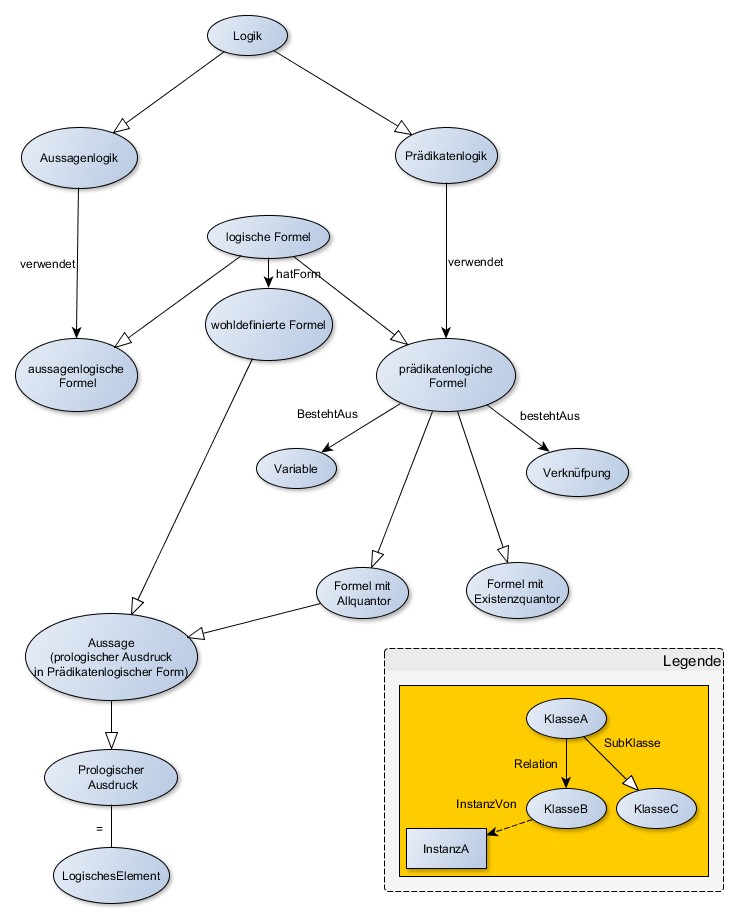
\includegraphics{bilder/formel_baum.png}}}
\caption{Vereinfachte Darstellung von Logik, rein mittels Klassen.\label{fig:prolog_logik_baum}\protect\footnotemark}
\end{figure}
\footnotetext{Eigene Darstellung mittels yEd.}

\newpage

Um auch Relationen abbilden zu können, wurde die Modellierung schliesslich mit Individuen erweitert. Dies erlaubte die Definition von Relationen zwischen diesen, was sich als Schritt in die richtige Richtung erweisen sollte.

\begin{figure}[H]
\centering \rotatebox{0}{\scalebox{0.3}[0.3]{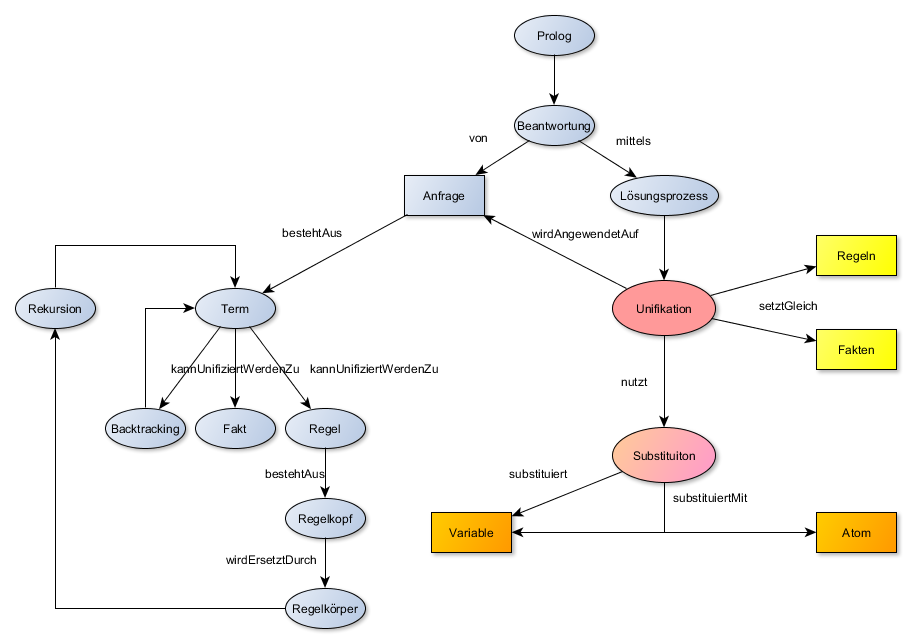
\includegraphics{bilder/loesungsprozess_baum.png}}}
\caption{Vereinfachte Darstellung eines Teils des Lösungsprozesses von Prolog, mittels Klassen, Individuen und Relationen.\label{fig:prolog_loesungsprozess}\protect\footnotemark}
\end{figure}
\footnotetext{Eigene Darstellung mittels yEd.}

Es wurde dann jeweils versucht konkrete Fragen aufgrund der erstellten Ontologie zu beantworten, wodurch Unvollständigkeiten in der Modellierung  sichtbar wurden. Diese zeigten sich zum Beispiel in Form von sehr umständlichen Abfragen um einfache Fakten zu erhalten. Details zu den gemachten Abfragen finden sich im Anhang~\ref{sec:anhang:sparql_beispiele}.

\begin{figure}[H]
\centering \rotatebox{0}{\scalebox{0.6}[0.6]{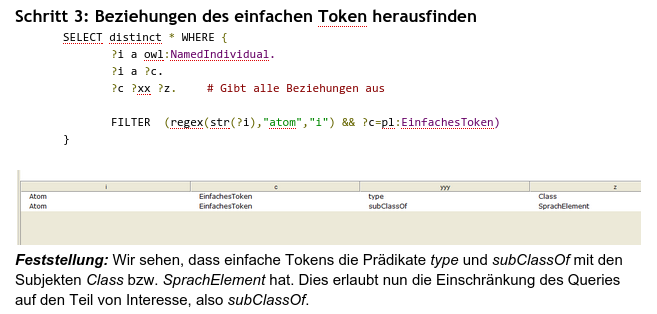
\includegraphics{bilder/sparql_beispiel.png}}}
\caption{Beispiel einer Abfrage der Ontologie mittels SPARQL.\label{fig:sparql_beispiel}\protect\footnotemark}
\end{figure}
\footnotetext{Eigene Darstellung mittels Stanford Protégé und Google Docs.}

Bei den genannten Mängeln handelte es sich nicht um Fehler. Grundsätzlich war es schwierig abzugrenzen bei welchem Detaillierungsgrad die Modellierung aufhören soll.So wurde schliesslich klar, dass bei einer zu feinen Granularität einer Modellierung, diese ins Uferlose gehen kann. Doch dies war nicht das Ziel, das Ziel war ein System zu schaffen, welches die Mächtigkeit dieser Art der Wissensmodellierung aufzeigt und damit Erfahrungen zu gewinnen. Daraufhin empfahl der Betreuer der Arbeit, Herr Dr.\ Eckerle, Literatur über Prolog als Grundlage bzw.\ Rahmen zu verwenden. Hierbei wurde auf das Buch \textit{Künstliche Intelligenz} von \textit{U. Lämmel} und \textit{J. Cleeve} zurückgegriffen~\cite{laemmel}. Herr Dr.\ Eckerle empfahl eine Beschränkung auf die Programmiersprache und deren Kernkonzepte, so wie sie auch im Buch beschrieben werden. Daraus resultierte eine verbesserte Modellierung der Ontologie von Prolog, mit Klassen, Relationen und Individuen.

\begin{figure}[H]
\centering \rotatebox{0}{\scalebox{0.15}[0.15]{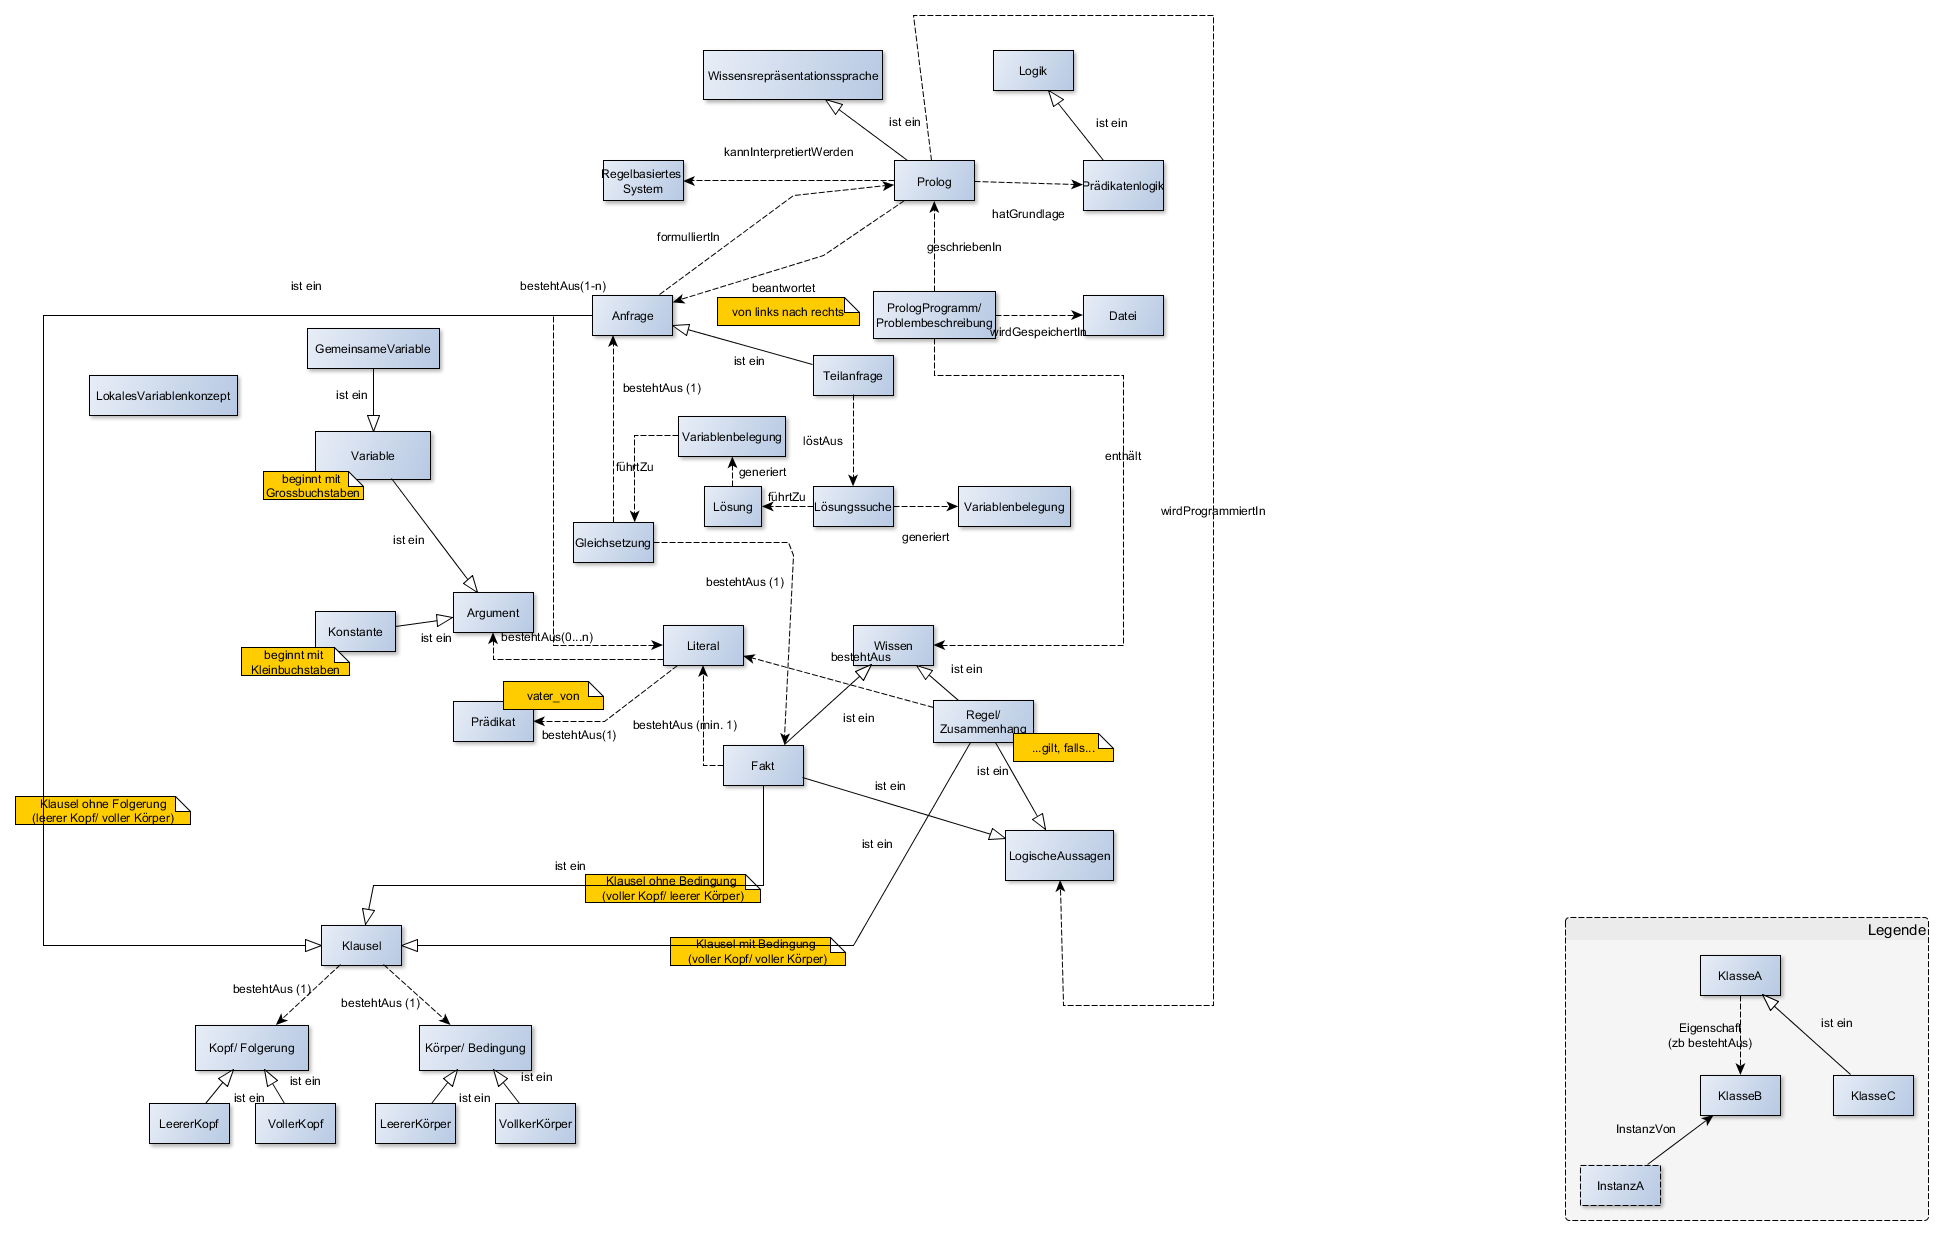
\includegraphics{bilder/prolog_baum.png}}}
\caption{Darstellung der Ontologie von Prolog, mit Klassen und Relationen (Individuen wurden der Übersicht halber bewusst weggelassen).\label{fig:prolog_baum}\protect\footnotemark}
\end{figure}
\footnotetext{Eigene Darstellung mittels yEd.}

Dies erlaubte jedoch nach wie vor keinen zusätzlichen Gewinn von Mehrwert in Form von Inferenz. Nach diversen Gesprächen mit Herrn Dr.\ Eckerle, stellte sich heraus, dass der Ontologie Regeln fehlen. Es wurde dann versucht mithilfe von Prolog das Konzept von Prolog abzubilden. Die Idee dahinter war, von der objektorientierten Denkweise loszukommen. Für die Autoren war es einfach nachzuvollziehen, dass und wie in Prolog Regeln verwendet werden. In Prolog wurde auch schnell deutlich, dass eine Abfrage auf Fakten (ohne Regeln) keinen Mehrwert bringt.

Nach diversen, erfolglosen Versuchen Regeln zu finden, wurde dies zuerst anhand einfacherer Modelle versucht. Zum Beispiel anhand eines Familienstammbaums. Mit diesem klassischen Beispiel wurde der Mehrwert der Wissensmodellierung mittels Ontologien sogleich erkannt.

\begin{figure}[H]
\centering \rotatebox{0}{\scalebox{0.15}[0.15]{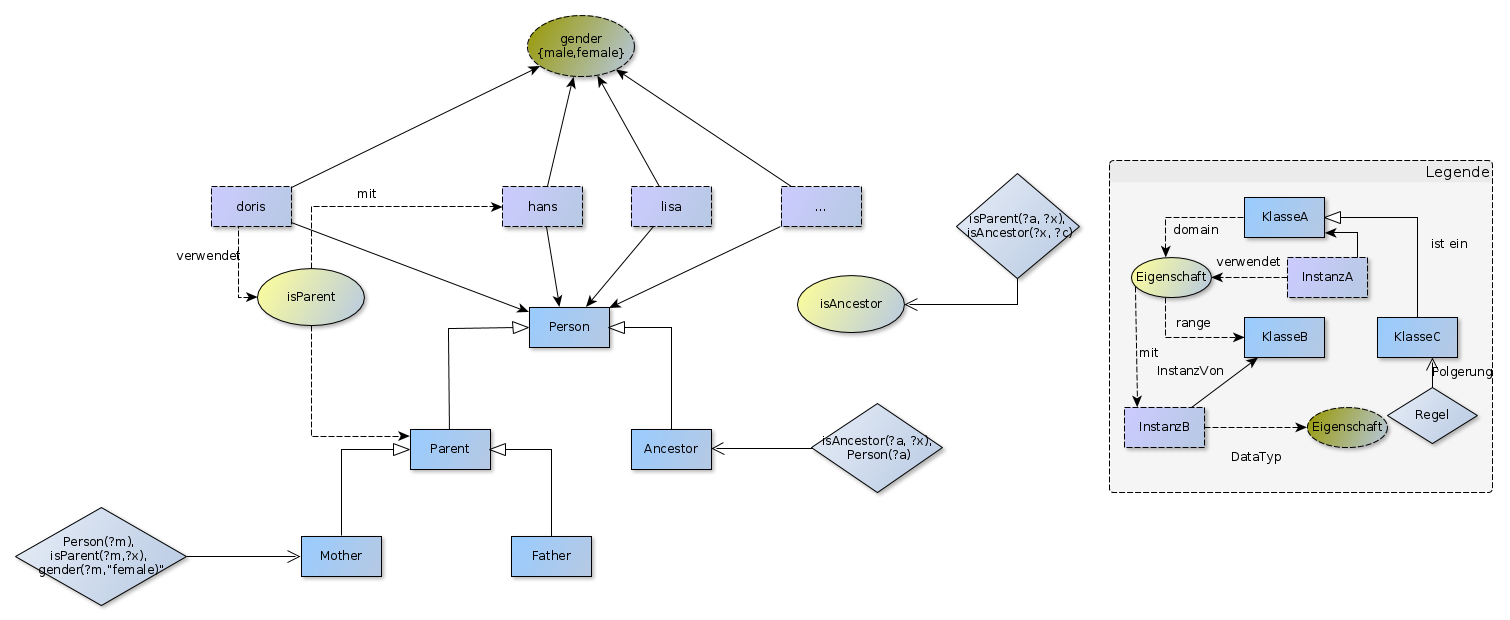
\includegraphics{bilder/familien_netz.png}}}
\caption{Ontologie eines Familienstammbaumes, mit Klassen, Individuen, Relationen und Regeln.\label{fig:familien_netz}\protect\footnotemark}
\end{figure}
\footnotetext{Eigene Darstellung mittels yEd.}

Es gelang nach dieser Erfahrung weiterhin nicht, Regeln für die eigentliche Wissensdomäne zu finden. Die Erkenntnis aus diesem Prozess war, dass die Abbildung von Prolog in einer Ontologie zwar möglich ist, jedoch eher in lexikalischer Form, was den Vorteil der Inferenz zu Nichte macht.

So kann beispielsweise gesagt werden, dass Prolog Unifikation auf Anfragen anwendet und dabei Regeln mit Fakten gleichsetzt. Dabei wird Substitution genutzt, welche Variablen mit Variablen und/oder Atomen substituiert. Dies wurde aber Grösstenteils in Form von Fakten abgebildet. Einige wenige Regeln konnten erzeugt werden.

Das damit abgebildete Wissen könnte aber auf eine einfachere und intuitivere Art mittels Fakten abgebildet werden. Somit ist der Mehrwert der Regel nichtig.

Nach eingehender Analyse kamen die Autoren zum Schluss, dass sich die gewählte Domäne nicht eignet, um die Mächtigkeit einer Ontologie und dem damit verbundenen Reasoning abzubilden. Für die Wissensmodellierung bzw. Expertensysteme eignen sich also eher Wissensdomänen, welche Probleme mit konkreten Objekten abbilden. Im Gegensatz dazu befindet sich die ursprünglich gewählte Domäne auf einer zu hohen Abstraktionsebene. Daher ist dort der konkrete Nutzen, in Form von Inferenz, nicht direkt sichtbar.

Wie der Name Expertensystem schon andeutet, werden diese in Fällen verwendet, bei denen ein Fachexperte notwendig ist. Dieser kann mit seinem Fachwissen Schlüsse ziehen und so zusätzliches Wissen generieren.

Daher wurde eine andere Wissensdomäne --- die Planung von Reisen --- gewählt. Dies geht bereits eher in die Richtung von Expertensystemen, wofür semantische Netze am ehesten geeignet scheinen.

Dieser Entscheidung gingen diverse Diskussionen und Versuche zur Wahl einer geeigneten Domäne voraus. So wurde zum Beispiel auch die Planung von Hochzeiten und medizinische sowie pharmazeutische Themengebiete in Betracht gezogen. Von diesen wurde jedoch abgesehen, da die Autoren in den Gebieten über zu wenig Fachwissen verfügen.

\begin{figure}[H]
\centering \rotatebox{0}{\scalebox{0.2}[0.2]{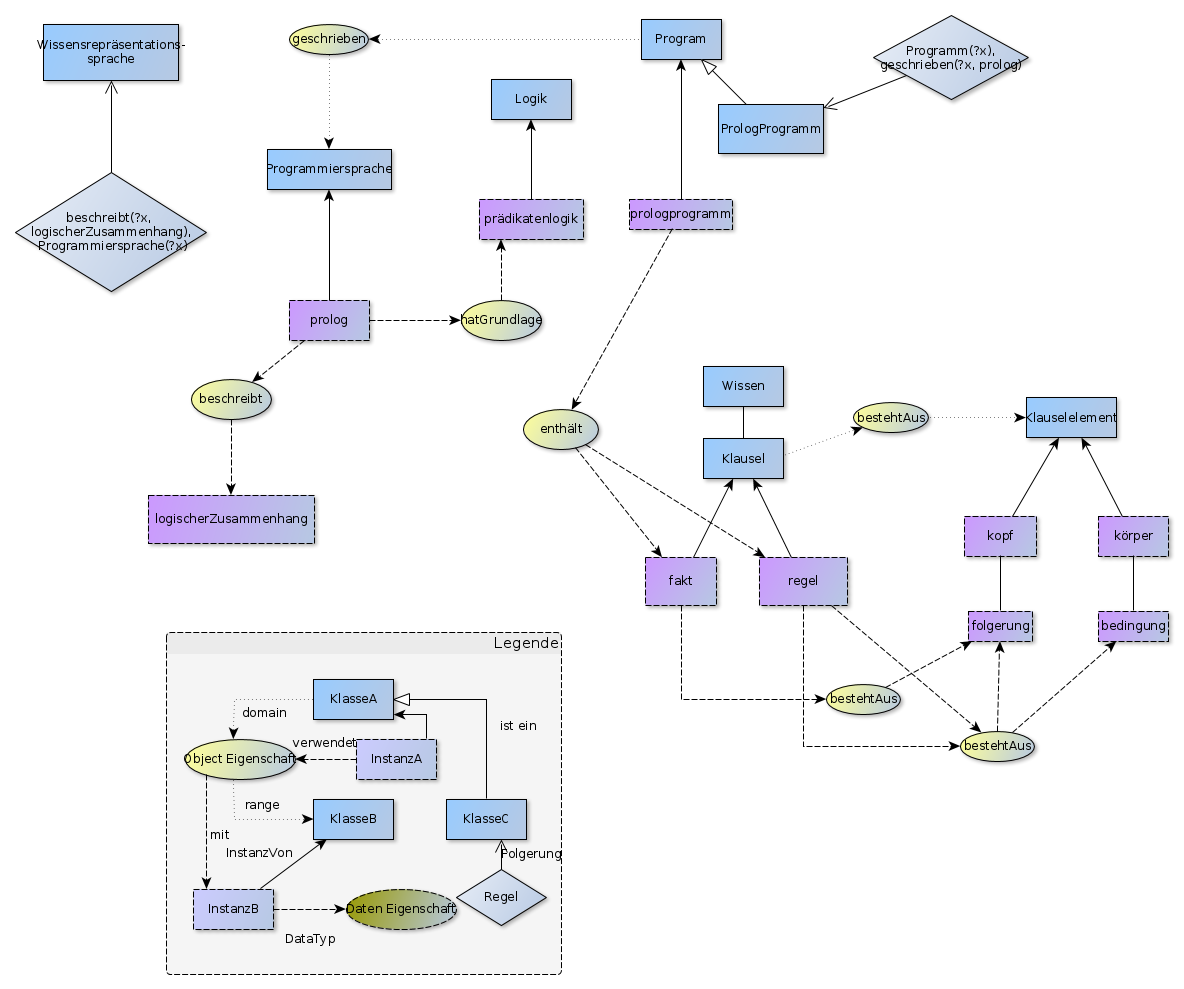
\includegraphics{bilder/prolog_netz.png}}}
\caption{Darstellung eines semantischen Netzes zur Abbildung von Prolog, mit Klassen, Individuen, Relationen und Regeln.\label{fig:prolog_netz}\protect\footnotemark}
\end{figure}
\footnotetext{Eigene Darstellung mittels yEd.}

\subsubsection{Modellierung der tatsächlichen Ontologie}
\label{sub:modellierung_der_ontologie_tatsaechliche}

Nach dieser Entscheidung wurde mit der Modellierung noch einmal beim Punkt null begonnen. Es konnte aber glücklicherweise auf den Erkenntnissen und Erfahrungen der vorigen Versuche aufgebaut werden.

Die Autoren entschieden sich anhand des gewonnen Wissens die Modellierung mittels konkreten Bespielen zu erarbeiten. Basierend auf diesen wurde die Ontologie erzeugt und stetig erweitert. Zur Veranschaulichung ein konkretes Beispiel:

\begin{lstlisting}[caption={Konkretes Beispiel einer Reiseplanung.},captionpos=b]
    Familie Muster plant einen eintägige Ausflug.
    Die Kinder sind in einem Alter in dem Sie immer beschäftigt sein müssen.
\end{lstlisting}

Im nachfolgenden Abschnitt findet sich eine Übersicht der Herleitung des Beispiels. Die Gedankengänge dahinter sind im Tutorial aufgeführt.

\newpage

Dies ergab eine noch sehr simple Ontologie, welche mit diesem semantischen Netz abgebildet werden kann:

\begin{figure}[H]
\centering \rotatebox{0}{\scalebox{0.5}[0.5]{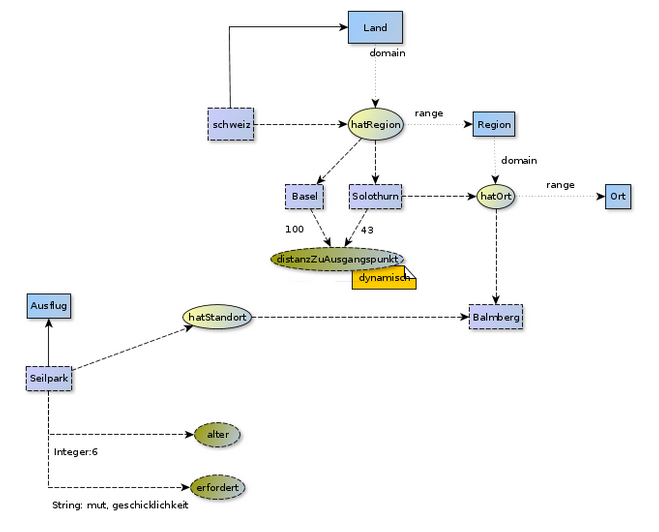
\includegraphics{bilder/famMuster.png}}}
\caption{Semantisches Netz für den Tagesausflug von Familie Muster.\label{fig:famMuster}\protect\footnotemark}
\end{figure}
\footnotetext{Eigene Darstellung mittels yEd.}

Mit der neu gewählten Wissensdomäne wurde auch der Sinn hinter der Verwendung von Regeln deutlich:
\begin{figure}[H]
    \centering \rotatebox{0}{\scalebox{0.5}[0.5]{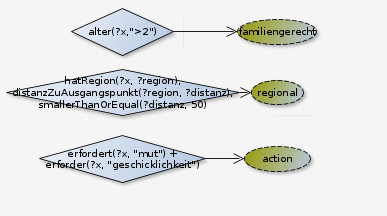
\includegraphics{bilder/famMusterRegeln.png}}}
    \caption{Regeln zum semantischen Netz für den Tagesausflug von Familie Muster.\label{fig:famMusterRegeln}\protect\footnotemark}
\end{figure}
\footnotetext{Eigene Darstellung mittels yEd.}

Aus der Modellierung konnten die folgenden Kriterien für die Abfrage abgeleitet werden:

\begin{itemize}
		\item familiengerecht
		\item action
		\item regional
\end{itemize}

Diese sind zugleich die Schlüsse der Regeln. Mit der richtigen SPARQL-Abfrage wird der Familie Muster schliesslich der Seilpark in Balmberg vorgeschlagen.

\begin{lstlisting}[caption={SPARQL-Abfrage um familiengerechte, regionale und actionreiche Ausflüge zu finden.},captionpos=b,language=SQL]
    SELECT
        *
    WHERE {
        ?object :familiengerecht true;
            :regional true;
            :action true.
        }
\end{lstlisting}


\begin{figure}[H]
\centering \rotatebox{0}{\scalebox{0.5}[0.5]{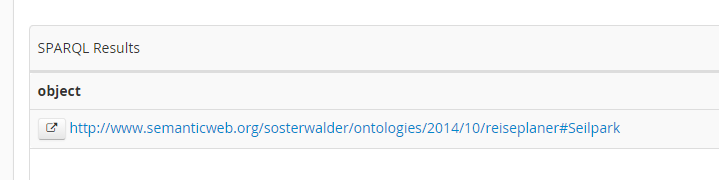
\includegraphics{bilder/famMusterOutput.png}}}
\caption{Ergebnis der Suche von Familie Muster.\label{fig:famMusterOutput}\protect\footnotemark}
\end{figure}
\footnotetext{Eigene Darstellung mittels yEd.}

In diesem ersten, bewusst sehr einfach gehaltenen Anwendungsfall, wird die Herangehensweise der Autoren sichtbar. Im Laufe von weiteren Beispielen wurde die Ontologie erweitert. So haben die Autoren zum Beispiel erst zu einem späteren Zeitpunkt eine Zeiteinheit eingeführt oder gemerkt, dass die Eigenschaft familiengerecht zu oberflächlich und pauschal betrachtet wurde. Diese wurde dahingehend geändert, dass die Eigenschaft Untereigenschaften beinhaltet, welche unterscheiden in welchem Alter die Kinder sind. Die gesamte Ontologie wird im~\autoref{sec:loesung_modellierung} genauer erläutert.

\subsection{Erstellung der Dokumentation zur Wissensmodellierung}
\label{subsec:dokumentation_wissensmodellierung}
Parallel zur Modellierung der Ontologie entstand ein Tutorial, welches aufzeigt, wie ein Knowledge Engineer vorgeht um eine Problemdomäne systematisch zu modellieren und formalisieren. Wie bereits zuvor erwähnt, wurde als Problemdomäne die Planung von Reisen gewählt. Das Tutorial findet sich im Anhang unter~\ref{sec:anhang:tutorial_dokument}.

\subsubsection{Aufbau des Tutorials}
\label{subsec:dokumentation_wissensmodellierung_aufbau}
Im Gegensatz zu herkömmlichen Tutorials enthält das in dieser Arbeit erstellte einen grossen Theorieanteil. Aus diesem Grund wurde das Dokument in drei Aspekte aufgeteilt.

Da es sich hierbei um eine wissenschaftliche Arbeit handelt, haben die Autoren entschieden in einem ersten Teil theoretisches Hintergrundwissen zur Wissensmodellierung bereitzustellen. So wird zum Beispiel erläutert was Expertensysteme sind, wie diese grafisch dargestellt werden können und welche Schreibweisen respektive Sprachen verwendet werden um eine Ontologie abzubilden und darauf Abfragen zu stellen.

\noindent\rule[1ex]{\textwidth}{1pt}
\begin{wrapfigure}[4]{l}{0.1\textwidth}
    \vspace{-18pt}
    
\includegraphics[width=0.1\textwidth]{bilder/owl.png}
\end{wrapfigure}
Durch das Symbol der Eule wird die zweite Herangehensweise im Dokument eingeleitet. Im jeweils danebenstehenden Abschnitt sind praktische Hinweise zur aktuellen Thematik aufgeführt.\\
\noindent\rule[1ex]{\textwidth}{1pt}

\noindent\rule[1ex]{\textwidth}{1pt}
\begin{wrapfigure}[4]{l}{0.1\textwidth}
    \vspace{-18pt}
    
\includegraphics[width=0.1\textwidth]{bilder/elephant.png}
\end{wrapfigure}
Der letzte Teil des Dokumentes, welcher durch das Symbol des Elefanten gekennzeichnet ist, verkörpert ein Tutorial im klassischen Sinne. Einem pragmatisch veranlagten Leser ist es so möglich, durch Folgen des Symbols, innerhalb von kurzer Zeit ein simples Beispiel eines Expertensystemes aufzubauen.\\
\noindent\rule[1ex]{\textwidth}{1pt}

\subsection{Erstellung der abschliessenden Dokumentation}
\label{subsec:abschliessende_dokumentation}
Mit der Erstellung der abschliessenden Dokumentation ist das hier vorliegende Dokument gemeint. Dieses wurde während der ganzen Projektarbeit stetig erweitert, auch um die bereits fertiggestellten Arbeiten zu reflektieren. Als Grundlage für das Dokument diente das bereits erwähnte Dokument, in welchem die Autoren ihre Erkenntnisse fortlaufend festhielten.

\chapter{Lösungsansatz}
\label{chap:loesungsansatz}

% Hier beschreiben Sie Ihren Lösungsansatz. Der Lösungsansatz ist ein Beschrieb auf hoher Abstraktionsebene. Beschreiben Sie, falls nötig, die zum Einsatz gekommenen Technologien nur dann, wenn die Beschreibung für das Verständnis der Arbeit unbedingt notwendig ist.
In der heutigen Zeit werden Ferien häufig per Internet gebucht. Was aber, wenn der Urlaub nicht einfach zwei Wochen an einem Ort stattfinden soll? Was, wenn der Kunde reisen möchte? Oder sonstige spezielle Wünsche hat? Für solche Anforderungen muss er auch heute noch ins Reisebüro um sich beraten zu lassen.

Um auch diesen Prozess zu automatisieren soll eine Ontologie erstellt werden, welche mithilfe von Eigenschaften, Kriterien und Regeln verschiedene Reisevorschläge machen kann.
Vorgehen
Damit dieses Ziel erreicht werden kann, muss zuerst eine Ontologie in Form von Klassen, Individuen, Relationen und Eigenschaften erstellt werden. Dies kann jedoch schnell ins Uferlose übergehen, wenn kein klarer Rahmen definiert ist. Daher wird anhand von exemplarischen Reisen die Ontologie schrittweise aufgebaut.

Konrekt werden Beispiele von Reisen mit diversen Anforderungen genannt, welche dann Stück für Stück modelliert werden, so dass schlussendlich eine vollständige Ontologie entsteht. Ein Beispiel solch einer Reise kann z.B. eine vierwöchige Abenteuerreise für Singles quer durch den Amazonas, verbunden mit einem abschliessenden Aufenthalt in einem Wellness-Ressort. Dabei darf das Budget beispielsweise eine gewisse Limite nicht überschreiten.

\chapter{Implementation}
\label{chap:implementation}

% In diesem Kapitel beschreiben Sie Ihre Lösung des Problems. Geben Sie dem Leser genügend Einblick in die Lösung, so dass er Ihre Arbeit entsprechend würdigen kann. Verwenden Sie aber Anhänge für Dinge, die hier nicht unbedingt bis ins letzte Detail verstanden werden müssen.

\section{Komponenten}
\label{sec:komponenten}

\subsection{Stanford Protégé}
\label{subsec:protege}

\subsection{Clark \& Parsia Stardog}
\label{subsec:stardog}

\subsubsection{Reasoner}
\label{ssubsec:reasoner}
Reasoner sind Komponenten, welche eine Folgerung von implizitem Wissen zulassen bzw.\ bieten. Es handelt es sich um eine Art ``Verstehen'' durch Maschinen. Man möchte also implizite Fakten finden, welche durch explizite Fakten in einer Ontologie definiert sind. 

Als Reasoner kommt Pellet zum Einsatz. Dabei handelt es sich um einen Reasoner, für die Sprache OWL-DL~\footnote{http://www.w3.org/TR/owl-ref/\#OWLDL}, welche wiederum eine Teilsprache von OWL darstellt. Eine komplette Unterstützung des OWL full Profils ist so nicht möglich, da dieses nicht entscheidbar ist, daher beschränkt sich die Umsetzung auf OWL DL\@. Pellet setzt dabei komplett die Spezifikation der WebOnt Arbeitsgruppe um. OWL-DL ist eine syntaktische Variante der Beschreibungslogik SHOIN (D).

\begin{figure}[htbp]
\centering \rotatebox{0}{\scalebox{0.5}[0.5]{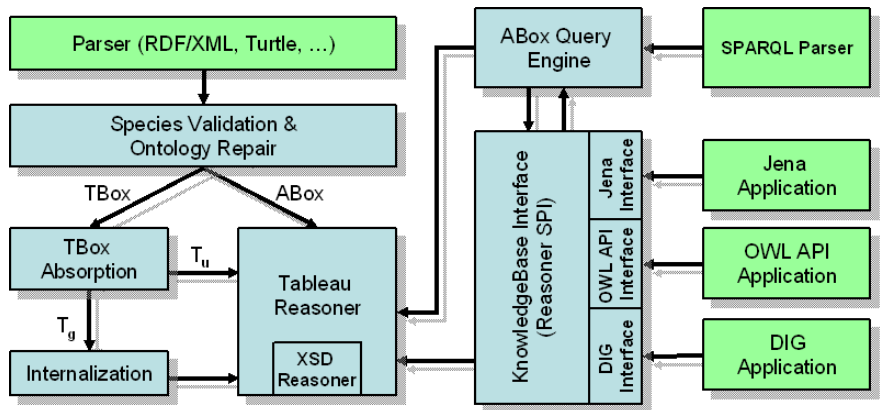
\includegraphics{bilder/pellet_komponenten.png}}}
\caption{Hauptkomponenten des Pellet-Reasoners.\label{fig:pellet_komponenten}\protect\footnotemark}
\end{figure}
\footnotetext{\cite[S. 6]{sirin:pellet05}}

\subsubsection{Beschreibungslogik}
\label{subsubsection:beschreibungslogik}
Beschreibungslogiken sind Formalismen um Wissen darzustellen, dabei sind sie eine Teilmenge der Prädikatenlogik. Sie stellen den Kern von Wissensrepräsentationssystemen dar, in dem sie eine Struktur für eine Wissensbasis und den damit verbundenen Methoden zur Folgerung bieten (vgl.~\cite{dl:baader2003}).

Die Struktur, welche Beschreibungslogiken als Wissensbasis bereitstellen, besteht aus einem Schema (Tbox, Regeln), sowie aus den Daten (Abox, Fakten).

Die Semantik von Beschreibungslogiken wird durch Interpretationen definiert:

\noindent\hspace*{16mm} $ I = (\Delta^I, \cdot^I) $

Dabei ist:
\begin{itemize}
\item $ \Delta^I $

    Die (Wissens-) Domäne (eine nicht leere Menge).

\item $ \cdot^I $

    Eine Funktion zur Interpretation von:
    \begin{itemize}
        \item Konzepten (Klassen, A)

            Wobei $ A^I $ eine Teilmenge von $ \Delta^I $ ist.
        \item Rollen (Eigenschaften, R)

            Wobei $ R^I $ eine binäre Relation auf $ \Delta^I $ ist.
        \item Individuen (i)

            Wobei $ i^I $ Element von $ \Delta^I $ ist.
    \end{itemize}
\end{itemize}

Die Funktion zur (Wissens-) Interpretation $ \cdot^I $ definiert, wie atomare Konzpte, Eigenschaften und Individuen zu interpretieren sind. Eine Interpretation, welche allen Axiomen einer Ontologie in Beschreibungslogik genügt ist ein Modell der Ontologie.

Eine Ontologie in Beschreibungslogik ist eine Menge von Termen und deren Relationen. Die Interpretation dieser Ontologie stellt als ein Modell dar, welches die Ontologie abbildet.

Die Pellet zu Grunde liegende Beschreibungslogik SHOIN (D) ist ein Kürzel und steht für:
\begin{itemize}
\item \textit{S}

ALC (Attributive Concept Language with Complements) mit einer transitiven Rolle. Bei ALC handelt es sich um die kleinste Beschreibungslogik, welche aussagenlogisch geschlossen ist (d.h.\ sie bietet, entweder implizit oder explizit, Konjunktion, Union und Negation von Klassen (-beschreibungen)). Eine Rolle entspricht einer Eigenschaft bzw.\ einem Prädikat in der Prädikatenlogik erster Stufe.

\item \textit{H}

    Rollenhierarchie (Sub-Eigenschaften), z.B. rdfs:subPropertyOf.

\item \textit{O}

    Nominal, z.B. Wochenden = {Samstag, Sonntag}.


\item \textit{I}

    Inverse Rolle (inverse Eigenschaft bzw.\ Prädikt).

\item \textit{N}

    Nummerische Einschränkung, z.B. >= hatKind 1.

\item \textit{(D)}

    Nutzung von Wertebereichen, Werten oder Datentypen.
\end{itemize}

(vgl.~\cite{dl:baader2003})

\subsubsection{Folgerung}
\label{subsubsection:folgerung}
Die W3C Spezifikation betreffend der Umsetzung eines Reasoners definiert zwei Arten von OWL Dokumentprüfungen: Prüfung auf korrekte Syntax sowie Prüfung der Konsistenz. Bei der Konsistenzprüfung geht es darum festzustellen, ob eine gegebene Eingabe anhand einer definierten Spezifikation syntaktisch korrekt ist. Jedoch macht eine reine Umsetzung der genannten Prüfungen wenig Sinn. Man möchte ja eine Ontologie möglichst effektiv nutzen können, zum Beispiel um indirektes Wissen abzuleiten.  Da OWL DL eine syntaktische Variante der Beschreibungslogik SHOIN (D) darstellt, liegt es nahe, mittels einem Reasoner folgende Methoden zur Inferenz zur Verfügung zu stellen:
\begin{itemize}
\item \textit{Konsistenzprüfung}

Stellt sicher, dass sich in der Ontologie keine gegenstätzlichen Fakten befinden. Konkret bedeutet dies anhand der OWL Semantik~\footnote{http://www.w3.org/TR/owl-semantics/}, dass die Konsistenz einer ABox in Bezug auf eine TBox geprüft wird.
\item \textit{Konzept-Erfüllbarkeit}

Stellt sicher, dass Objekte einer Klasse instanziert werden können. Ist dies nicht der Fall, so ist die Ontologie inkonsistent.
\item \textit{Klassifikation}

Berechnet die Relationen zwischen Subklassen, stellt also die Klassenhierarchie auf. Dies ermöglicht das Abfragen der Ontologie.
\item \textit{Gewinnung von Erkenntnissen}

Findet die spezifischste Klasse eines Objektes, leitet also den direkten Typ jedes Objektes ab.
\end{itemize}
(vgl. \citet[S. 1 und 2]{sirin:pellet05})

Bei der eigentliche Komponente, welche in Pellet zur Folgerung eingesetzt wird, handelt es sich um den Tableau Reasoner, welcher den gleichnamigen Algorithmus verwendet. Dieser reduziert ein Problem der Folgerung auf ein Problem der Konzept-Erfüllbarkeit, wobei er eine Interpretation sucht, welche die gefragten Konzepte erfüllt. Solch eine Interpretation wird inkrementell als eine Art Tafel (eben, Tableau) aufgebaut.

Nachfolgend ein Beispiel, gegeben sei:
$ Prolog \subseteq LogischeProgrammiersprache, LogischeProgrammiersprache \subseteq Programmiersprache $
Man stellt nun folgende Anfrage:
$ if Prolog \subseteq Programmiersprache $

Der Prozess der Folgerung findet nun wie folgt statt:
\begin{itemize}
    \item Testen, ob ein Individuum existiert, welches eine logische Programmiersprache, aber keine Programmiersprache ist. Man möchte also die Erfüllbarkeit des Konzeptes $ C_0 = (Prolog \sqcap \neg Programmiersprache) $ testen.
    \item $ C_0(x) \Rightarrow Prolog(x), (\neg Programmiersprache)(x) $
    \item $ Prolog(x) \Rightarrow LogischeProgrammiersprache(x) $
    \item $ LogischeProgrammiersprache(x) \Rightarrow Programmiersprache(x) $
        $ \Rightarrow $ Konflikt!
\end{itemize}
Wie ersichtlich ist, ist das Konzept $ C_0 $ nicht erfüllbar, die Anfrage $ Prolog \subseteq Programmiersprache $ trifft also innerhalb der gegebenen Ontologie zu. Der Beweis wird mittels Kontradiktion erbracht.

Der generelle Prozess der Folgerung läuft wie folgt ab:
\begin{itemize}
    \item Umwandlung eines Konzeptes bzw.\ der Konzepte in die negierte Normalform (NNF), die Negation $ \neg $ befindet sich vor Konzeptnamen.
    \item Ablegen des umgewandelten Konzeptes als $ C_0 $.

        Der Algorithmus hat also die Datenbasis (Abox) $ A_0 = {C_0(x_0)} $
    \item Regeln zur Transformation auf die Datenbasis (Abox) so weit als möglich anwenden.
    \item Wurde eine gültige Datenbasis (Abox) gefunden, so ist $ C_0 $ erfüllbar.
    \item Wurde keine gültige Datenbasis unter Berücksichtigung aller (Such-) Pfade gefunden, so ist $ C_0 $ nicht erfüllbar.
\end{itemize} (vgl.~\cite{horrocks2002} und~\cite{horrocks2005})

\chapter{Fazit und Ausblick}
\label{chap:fazit}

% In diesem Kapitel legen Sie Ihre kritische Betrachtung Ihrer Arbeit dar. Zeigen Sie, was Sie erreicht haben. Hinterfragen Sie das Ergebnis auf objektive Art und Weise.

Im Kapitel Lösung wurde bereits festgestellt, dass sämtliche Ziele der Arbeit erreicht wurden. Dabei ist wichtig, dass wir im Laufe der Arbeit die Problemdomäne ändern geändert haben. Die ursprünglich gewählte Domäne des Erlernens des Programmierens anhand der Programmiersprache Prolog stellte sich als nicht geeignet heraus.

Als wir dieses Gebiet auswählten, wussten wir noch zu wenig über die Wissensmodellierung mittels Ontologien. So war uns nicht bewusst, dass sich diese vor allem für solche Gebiete eignet, in denen viele Fakten vorhanden sind. Das Erlernen des Programmierens anhand Prolog ist ein sehr theoretisches Gebiet mit Abläufen und Verallgemeinerungen. Im Gegensatz ist die das Planen von Reisen viel besser dazu geeignet. Damit war es uns möglich die verschiedenen Spezialitäten eines Expertensystems herauszufinden und die Mächtigkeit von semantischen Datenbanken aufzuzeigen.

Bei unserer Arbeit lag der Fokus nicht auf einem genau definierten Endprodukt. Viel mehr stand der gesamte Prozess der Wissenserarbeitung im Vordergrund. Ein wichtiger Teil war die Modellierung einer Ontologie. Hierbei war es schwierig ein sinnvolles, allgemeines Vorgehen zu finden und definieren. So sehen wir die verschiedenen Schwierigkeiten, auf welche wir während des Prozesses gestossen sind, nicht als Nachteil sondern als Erfahrung an.

Wir haben uns bewusst für ein für uns eher unbekanntes Thema der Thesis entschieden. Dies vor allem, weil wir in der Erarbeitung der Bachelor Thesis eine Chance sahen zu forschen und zu experimentieren. In der Berufswelt, welche jetzt auf uns wartet wird dies wahrscheinlich nur noch begrenzt möglich sein. Uns ist aber erst beim Reflektieren der Arbeit richtiggehend bewusst geworden, dass wir ein Themengebiet gewählt haben bei dem wir ausser einigen simplen Grundlagen alles neu erarbeiten mussten. Es war uns nur sehr bedingt möglich, vorhandenes Wissen anzuwenden. Dies führte zu einer sehr spannenden und intensiven Arbeit.

Als Vorbereitung für die Bachelor Thesis besuchten wir das Wahlpflichtfach Künstliche Intelligenz. In diesem Modul, hatten wir die Möglichkeit uns zumindest oberflächlich mit der Programmiersprache Prolog auseinander zusetzten. Aus diesem Grund entstanden regelmässige Vergleiche zwischen Expertensystemen welche auf Ontologien aufbauen und Prolog. Ein eindeutiger Vorteil von Wissensmodellierung auf Basis von Ontologien mittels OWL ist, dass es einige Werkzeuge gibt, welche die Modellierung unterstützten. So können mithilfe von Protégé auf eine übersichtliche Art Fakten abgebildet werden. Dies wird noch unterstützt durch die Tatsache, dass in OWL eine klare Klassen - Eigenschaft - Beziehungstrennung bestet. Dies führt zu einem Raster welches zu einer verbesserten Trennung führt. Die XML ähnliche Syntax ermöglicht zudem eine\\ 

%- Wissensmodellierung hat vor und nachteile:\\
%   Vorteile: html schnittstelle; mit vorhandenen Werkzeugen wird es übersichtlicher (Protege)\\
%   Nachteile: Regeln mit Indiviuen nicht möglicht; Rechnen nur eingeschränkt möglich\\
%- Struktur der ARbeit sinnvoll; mit erarbeiten der Grundlagen und Praktischer Umsetztung
%Vorteile und Nachteile
%+ Sehr klare Trennung Eigenschaften, Klassen und Relationen => klares Raster
%+ Verwendung von Logik / Ableitung von Regeln
%+ Mischform UML und Prolog
%- Abläufe sind sehr schwer abzubilden
%Ein grosser Vorteil im Vergleich zu anderen Expertensystemen ist sicher, dass die OWL / XML Schreibweise gut verarbeitet werden kann und es sich so anbietet HTML-Schnittstellen zu genieren und zu nutzen.  (TODO soll hier gesagt werden was?). 

% - Zusammenfassung des Resultats
% - Würdigung des Resultats
% - Evtl. Empfehlungen zum weiteren Vorgehen

\section{Ausblick}
\label{sec:fazit_subchap}
Bei dem aktuellen Modell der Ontologie sowie der Benutzeroberfläche handelt es sich um einen Nachweis der Machbarkeit in Form von Prototypen. Der Funktionsumfang dieser beschränkt sich daher nur auf das Nötigste und entspricht nicht einer realen Anwendung.

Wollte man das Umgesetzte einer praxisrelevanten Anwendung nutzen, so müsste dies erweitert werden. Die Ontologie verfügt nur über einige wenige, exemplarische Entitäten. Um interessante Abfragemöglichkeiten bieten zu können, wäre sicherlich eine starke Erweiterung der Ontologie nötig.

Weiter könnte die Anwendung mit Benutzerprofilen versehen werden, welche den Standort des Benutzers speichern. Mittels einer Geoinformationssoftware könnte so die Distanz zu Entitäten (z.B. Restaurants und Ausflüge) dynamisch berechnet werden.

Das Modell unterstützt aktuell nur eine Zeitauflösung von einem halben Tag, einem ganzen Tag sowie mehr als einem Tag. Eine feinere Zeitauflösung, etwa in Form von Fliesskommawerten, liesse eine genauere Planung von Reisen zu. Dies müsste jedoch in Form von Applikationslogik und nicht durch den Reasoner umgesetzt werden, da dieser, wie im Tutorial erwähnt, keine Bedingungserfüllungsprobleme lösen kann.



\chapter{Schlussbemerkung}
\label{chap:schlussbemerkung}

% Falls vorhanden, können Sie hier Ihren Dank ausprechen. Sie können hier auch Kommentare zum Umfeld der Arbeit abgeben, zum Beispiel über die Betreuung oder den Auftraggeber.

%---------------------------------------------------------------------------

% Selbständigkeitserklärung
%---------------------------------------------------------------------------
\cleardoublepage{}
\phantomsection{}
\addcontentsline{toc}{chapter}{Selbständigkeitserklärung}
\chapter*{Selbständigkeitserklärung}
\label{chap:selbstaendigkeitserklaerung}

\vspace*{10mm} 

Ich/wir bestätige/n, dass ich/wir die vorliegende Arbeit selbstständig und ohne Benutzung anderer als der im Literaturverzeichnis angegebenen Quellen und Hilfsmittel angefertigt habe/n. Sämtliche Textstellen, die nicht von mir/uns stammen, sind als Zitate gekennzeichnet und mit dem genauen Hinweis auf ihre Herkunft versehen. 

\vspace{15mm}

\begin{tabbing}
xxxxxxxxxxxxxxxxxxxxxxxxx\=xxxxxxxxxxxxxxxxxxxxxxxxxxxxxx\=xxxxxxxxxxxxxxxxxxxxxxxxxxxxxx\kill
Ort, Datum:		\> [Biel/Burgdorf], \versiondate \\ \\ 
Namen Vornamen:	\> [Test Peter] 	\> [Müster Rösä] \\ \\ \\ \\ 
Unterschriften:	\>......................................\>......................................\\
\end{tabbing}

%---------------------------------------------------------------------------

% Glossary
%---------------------------------------------------------------------------
%\cleardoublepage
\phantomsection{}
\addcontentsline{toc}{chapter}{Glossar}
\renewcommand{\glossaryname}{Glossar}
\printglossary{}
%---------------------------------------------------------------------------

% Bibliography
%---------------------------------------------------------------------------
%\cleardoublepage
%\phantomsection{}
%\addcontentsline{toc}{chapter}{Literaturverzeichnis}
\bibliographystyle{unsrtdin}
\bibliography{datenbanken/bibliography}{}
%---------------------------------------------------------------------------

% Listings
%---------------------------------------------------------------------------
%\cleardoublepage
\phantomsection{}
\addcontentsline{toc}{chapter}{Abbildungsverzeichnis}
\listoffigures
%\cleardoublepage
%\phantomsection{}
%\addcontentsline{toc}{chapter}{Tabellenverzeichnis}
%\listoftables
%---------------------------------------------------------------------------

% Index
%---------------------------------------------------------------------------
%\cleardoublepage
%\phantomsection{}
%\addcontentsline{toc}{chapter}{Stichwortverzeichnis}
%\renewcommand{\indexname}{Stichwortverzeichnis}
%\printindex
%---------------------------------------------------------------------------

% Attachment:
%---------------------------------------------------------------------------
\appendix
\settocdepth{section}
\begin{titlepage}


    \clearpage
    \vspace*{\fill}
    \begin{center}
        \begin{minipage}{.6\textwidth}
            \fontsize{26pt}{28pt}\selectfont
            Anhang
        \end{minipage}
    \end{center}
    \vfill % equivalent to \vspace{\fill}
    \clearpage


\end{titlepage}

\newpage 

% In den Anhang fügen Sie ein:
%  * Details des Projektpans, falls vorhanden
%  * Resultate und Zwischenresultate in Funktion der Projektiterationen
%  * Pflichtenheft / Anforderungsspezifikation (Stand Ende dritter Woche)
%  * Angaben zum Projektrepository
%  * Sitzungsprotokolle, falls vorhanden
%  * Weiterführende Erläuterungen zu den verwendeten Technologien, falls nötig
%  * Benutzerhandbuch, falls vorhanden und sinnvoll, es hier aufzulisten
%  * Installations- und Betriebsdokument, falls vorhanden und sinnvoll, es hier aufzulisten
% Unterlassen Sie das Anfügen von Listings.

\appendix

\section*{Anforderungen}
\label{sec:anhang:anforderungen}
\href{anhang/anforderungen.pdf}{Anforderungsdokument}

\section*{Beispiele}
\label{sec:anhang:sparql_beispiele}
\href{anhang/schnipsel.pdf}{Dokument mit diversen Abfragebeispielen}

\section*{Dokumentation Wissensmodellierung}
\label{sec:anhang:tutorial_dokument}
\href{../Tutorial/template.pdf}{Dokumentation Wissensmodellierung}

\section*{Dokumentation BTI7302 --- Projekt2}
\label{sec:anhang:projekt2}
\href{../Extern/EigeneDokumente/DokumentationProjekt2.pdf}{Dokumentation BTI7302 - Projekt2}

\section*{Arbeitsjournal}
\label{sec:anhang:journal}
TODO:\@ Journal hier einfügen.

\section*{Benuterhandbuch}
\label{sec:anhang:handbuch}
TODO:\@ Handbuch hier einfügen.

\section*{Grafiken}
\label{sec:anhang:grafiken}
TODO:\@ Grafiken hier einfügen.

\section*{Reiseplaner}
\label{sec:anhang:reiseplaner}
TODO:\@ Reiseplaner hier einfügen.

%---------------------------------------------------------------------------

%---------------------------------------------------------------------------
\end{document}
